\chapter{Integration in a Neo4j}

In this section it is described how \cite[Customization Contraction Hierarchies]{CCH} is integrated into Neo4j.
CCH arguments the input graph, which means it inserts arcs, so called shortcuts, that do not belong to the original data.
We want to keep the change to the input graphs as little as possible we decided to not insert any arc into the graph that is stored inside the neo4j database, but introduce another graph data structure, the index graph.
%Through that decision we get full control over the data structure so we can decide how to store it.
The mapping between the index and the input graph, that resides in the database, is achieved by the rank property.
The rank property is set to the input and the the index graph at contraction time.
Through this we achieve a unique mapping between $G$ and $G'$.
This gives yet another two advantages.
One is that we get full control about the graph representation which is helpful to efficiently store and read the index graph for the disk.
Another is that it makes it easier to later on port the idea to another graph database manufactures.
Additionally to mention here is that the plugin documentation Neo4j provides is quite incomplete. 
Sometimes it only helps to reverse engineer their code as it always stops at the point which could get interesting. 
Presumably a support marketing strategy. 

\section{Index Graph Data Structure}\label{sec:index_graph}

\begin{figure}
    \begin{tikzpicture}
    \begin{class}[text width=0.5\linewidth]{Vertex}{0,0}
        \attribute{+ rank : int}
        \attribute{+ inArcs : Map<Vertex, Arc>}
        \attribute{+ outArc : Map<Vertex, Arc>}
        \operation{+ Vertex(rank: int)}
        \operation{+ addArc(other: Vertex, middle: Vertex, weight: int, hopLength:int) }
      \end{class}
\end{tikzpicture} 
    \begin{tikzpicture}
    \begin{class}[text width=0.5\linewidth]{Arc}{0.5\linewidth, 0}
      \attribute{+ start : Vertex}
      \attribute{+ end : Vertex}
      \attribute{+ middle : Vertex}
      \attribute{+ weight : int}
      \attribute{+ hopLength: int}
      \operation{+ Arc(start: Vertex, end: Vertex, weight: int, middle: Vertex, hopLength: int) }
      \operation{+ other(vertex: Vertex): Vertex}
    \end{class}
\end{tikzpicture}
    \caption{Index Graph}
    \label{uml:index_graph}
\end{figure}

The index graph data structure is neither a adjacency list nor adjacency matrix.
There is a vertex object that has two hash tables.
One for incoming arc and one for outgoing arcs.
The hash tables keys are of type vertex and the value is the arc.
An arc has a reference to its start vertex and one to its end vertex as shown in figure \ref{uml:index_graph}.
This also means we cannot construct them all at once, but need a function which initializes the graph, because we have a circular reference.
Our solution if you want to initialize such a graph, for an id pair that represents arc or from relationships that come from neo4j is as follows: We iterate over all id pairs, create all vertices that we have not seen so far an push them to a hash table.
Then we create the arc and attach the vertices to it.
These vertices we get from the hash table.
Finally we add the arc to its start and end vertex.
\\
A disadvantage of this model could be that some modern hardware optimization that exist for arrays do not match with this data structure.
Due to paging algorithms as described in \cite[Modern Operatins Systems]{andrew2015modern} the values of an array are stored sequentially in main memory.
When one value of an array is accessed by the CPU, modern hardware reads subsequent values into the CPU-cache because they most probably reside inside the same main me page.
The model of the index graph is a linked data structure, a bit like a linked list.
The elements of a linked list are contained somewhere in main memory.
There is no guarantee that subsequent values have any spacial proximity.
Therefore the just explained luckiness will not occur.
\\ % cite some paper to this topic
However, this makes the the graph traversal easy.
Additional it makes it very efficient to explore the neighborhood of a vertex.
There is no array traversal to find a vertex and only one hash table lookup for finding an arc of a vertex.
Test on a small graph, which represents the road network of Oldenburg, show that cch queries can be answered in less than one millisecond, which is close to what we tested with the original cch application.

\section{The Mapping}\label{sec:mapping}
\begin{figure}
    \centering
    \begin{tikzpicture}[node distance={15mm}, main/.style = {draw, circle}]
 
    \node[main, align=center] (x3) at (0,4) {id:23, labels:\{\\Location,…\}, \\props:\{\\rank:3,…\}};
    \node[main, align=center] (x2) at (12,2) {id:22, labels:\{\\Location,…\}, \\ props:\{\\rank:2,…\}};
    \node[main, align=center] (x1) at (6, 0) {id:21, labels:\{\\Location,…\},  \\ props:\{\\rank:1,…\}};
    
    \draw[ -Stealth] (x2) -- node[rectangle,draw, fill=white,  align=center] {:ROAD \\ weight:1.0}(x1);
    \draw[ -Stealth] (x1) -- node[rectangle,draw, fill=white,  align=center] {:ROAD \\ weight:1.0} (x3);
    \draw[dashed, -Stealth] (x2) -- (x3);

    \draw (0,-2) -- (10,-2);
    \draw (0,-2.5) -- (10,-2.5);
    \draw (0,-3) -- (10,-3);
    \draw (0,-3.5) -- (10,-3.5);
    \draw (0,-4) -- (10,-4);

    \draw (0,-2) -- (0,-4);
    \draw (2.5,-2) -- (2.5,-4);
    \draw (5,-2) -- (5,-4);
    \draw (7.5,-2) -- (7.5,-4);
    \draw (10,-2) -- (10,-4);

    \node[align=center] at (1.25, -2.25) {\textbf{start rank}};
    \node[align=center] at (3.75, -2.25) {\textbf{end rank}};
    \node[align=center] at (6.25, -2.25) {\textbf{middle rank}};
    \node[align=center] at (8.75, -2.25) {\textbf{weight}};

    \node[align=center] at (1.25, -2.75) {2};
    \node[align=center] at (3.75, -2.75) {3};
    \node[align=center] at (6.25, -2.75) {1};
    \node[align=center] at (8.75, -2.75) {2.0};

    \node[align=center] at (1.25, -3.25) {1};
    \node[align=center] at (3.75, -3.25) {3};
    \node[align=center] at (6.25, -3.25) {-1};
    \node[align=center] at (8.75, -3.25) {1.0};

    \node[align=center] at (1.25, -3.75) {2};
    \node[align=center] at (3.75, -3.75) {1};
    \node[align=center] at (6.25, -3.75) {-1};
    \node[align=center] at (8.75, -3.75) {1.0};

\end{tikzpicture}
    \caption{mapping}
    \label{fig:mapping}
\end{figure}

The in memory data structure of neo4j is similar to the just explained index graph data structure in section \ref{sec:index_graph}.
A \textit{node} has a collection of \textit{relationships} and a \textit{relationship} has a reference to its \textit{start node} and \textit{end node}.
As neo4j is a full blown property graph, nodes and relationships contain a lot of other information.
A node has a collection of \textit{labels}, relationship has a \textit{type}.
The class \textit{Node} and the class \textit{Relationship} 
are both derived from the class \textit{Entity} which also has a collection of properties as well as an id that is managed by the database system.
Note that, as of version Neo4j 5.X, this id can change over time and should not be used to make mappings to external systems.
Additionally worth to mentioning here is that the Neo4j system shifted its id concept as it moved from major release 4 to 5.
Until major release 4 every entity had a unique integer identifier.
Since major release 5 every entity has a string identifier which is a UUID and the old \textit{id} identifier isn't guaranteed to be unique anymore.
It is deprecated and marked for removal.
\\
As just explained there are lot of information in this data structure.
A lot of information we don't need.
Looking at figure \ref{fig:mapping} we only want to keep track of the information that is needed for the CCH index.
Additionally as disks are divided  into blocks and sectors we want to flatten the graph, which in memory more looks like a tree, to a structure that looks like a table.
Therefore we decided that the disk data structure only consists of arcs $\bigcirc A$.
A DiskArc $a \epsilon \bigcirc A$ consists of four values, 
the \textit{start rank}, the \textit{end rank}, the \textit{start rank} and the \textit{weight} .
The middle node is set $-1$ in case that this arc, is an arc of the input graph.
We will get two arc sets $\bigcirc A_\downarrow$ for the downwards graph and $\bigcirc A_\uparrow $ for the upwards graph.
$\bigcirc A_\downarrow$ contains all downward arc which are needed for the backward search and $\bigcirc A_\uparrow$ contains all upwards arcs that are needed for the forward search.
\\
During the the contraction every node gets a rank assigned.
This rank is the only change that is made to the Neo4j data structure and it's the mapping identifier between the input graph $G$ and the index graph $G'$.
$G'$ will then be used to generate $\bigcirc A_\downarrow$ and $\bigcirc A_\uparrow$.


\section{How to Store the Index Graph}\label{sec:how_to_store}

\begin{figure}
    \centering
    \begin{tikzpicture}[node distance={15mm}, main/.style = {draw, circle}]
    
    \draw (-7,6) rectangle (-1,7);
    \draw (-5.5,6) -- (-5.5,7);
    \draw (-4,6) -- (-4,7);
    \draw (-2.5,6) -- (-2.5,7);
    \node at (-6.25, 6.5) {from};
    \node at (-4.75, 6.5) {to};
    \node at (-3.25, 6.5) {middle};
    \node at (-1.75, 6.5) {weight};

    \draw [decorate,decoration = {brace, amplitude=5pt}] (-7,7.1) --  (-5.5,7.1);
    \draw [decorate,decoration = {brace, amplitude=5pt}] (-5.5,7.1) --  (-4,7.1);
    \draw [decorate,decoration = {brace, amplitude=5pt}] (-4,7.1) --  (-2.5,7.1);
    \draw [decorate,decoration = {brace, amplitude=5pt}] (-2.5,7.1) --  (-1,7.1);
    \node[ align=center] at (-6.25, 7.8) {32 bit  \\ integer};
    \node[ align=center] at (-4.75, 7.8) {32 bit  \\ integer};
    \node[ align=center] at (-3.25, 7.8) {32 bit  \\ integer};
    \node[ align=center] at (-1.75, 7.8) {32b bit \\ integer};

    \draw [decorate,decoration = {brace, amplitude=5pt}] (-1,5.9) --  (-7, 5.9);
    \node at (-4, 5.5) {16 byte disk arc};

    \draw[dashed, -Stealth] (-1,7) -- (0, 6.7);
    \draw[dashed, -Stealth] (-1,6) -- (0, 6.3);
    
    
    \draw (0,7) -- (4,7);
    \draw[dashed] (0,6) -- (4,6);
    \draw[dashed] (0,5) -- (4,5);
    \node at (4.5,5) {0};
    \node at (4.5,1) {1};
    \draw (0,3) -- (5,3); 
    \draw[dashed] (0,2) -- (4,2);
    \draw[dashed] (0,1) -- (4,1);
    \draw[out=60, in=-120] (0,0) to (4, 0);
    \draw (0,0) -- (0,7); 
    \draw (4,0) -- (4,7); 
    \node at (2, 6.5) {disk arc};
    \node at (2, 5.5) {disk arc};
    \node[rotate=90, font=\Large] at (2, 4) {. . . . .};
    
    \node[rotate=-90] at (5.85, 5) {disk block};
    \draw [decorate,decoration = {brace, amplitude=10pt}] (5.2,7) --  (5.2,3);
\end{tikzpicture}
\caption{Disk Block}
    \label{fig:disk_block}
\end{figure}

After generating the index graph $G'$, we now want to store them as efficiently as possible to the disk.
To refine the definition of a disk arc.
It consist of four $4 Byte$ signed integer values \textit{start rank}, the \textit{end rank}, the \textit{start rank} and the \textit{weight} as you can see in figure \ref{fig:disk_block}.
\\
This 16 Byte disk arcs are collected to disk blocks.
The size of a block can be set as parameter but has two lower bounds.
At first a disk block should not be smaller as the block size of the file system beneath as this is the smallest unit once can gets and it would be a wast of space.
Therefore it should also be a multiple of the system disk block size.
The second lower bound is the maximum degree that exists in the index graph after the contraction, as all arcs of one vertex, as all upward arcs a vertex have to be stored int the same disk block.
This applies for the downward arcs, too.

\begin{equation*}
    max(d_{\uparrow max}(v), d_{\downarrow max}(v)) \leqslant  \frac{diskBlockSize}{16}  
\end{equation*}

\subsection{Persistance Order}\label{sec:persistanceOrder}

\begin{algorithm}
    \caption{DFS in StoreFunction}
    \begin{algorithmic}
        \label{alg:store_dfs}
        \Procedure{store()}{}
        \While{stack $\neq \emptyset$}
            \If{stack.peekFirst().hasNext()}
                \State $\text{vertex} \gets \text{stack.peekFirst().next()}$
                \If{$\lnot$ positionWriter.alreadyWritten(vertex)}
                    \State position $\gets$ arcWriter.write(vertex)
                    \State positionWriter.write(vertex, position)
                    \State stack.addFirst(neighbors(vertex))
                \EndIf
            \Else
                \State stack.pollFirst()
            \EndIf
        \EndWhile
        \EndProcedure      
    \end{algorithmic}
\end{algorithm}

As the disk arcs are later on is used for the CCH search, we want to sequentially write them in a way that provides a high spatial proximity of vertices that are likely to get requested together.
Here we will adopt the idea of \cite[Mobile Route Planning]{Sanders}.
In the transformation form $G'$ to its disk arcs $\bigcirc A_\uparrow$ and $\bigcirc A_\downarrow$ we do a simple depth first search on all ingoing arcs on the target rank to determine the order for $\bigcirc A_\uparrow$.
We provided the algorithm for that in algorithm \ref{alg:store_dfs}.
As you can see in figure \ref{fig:store_function}, the StoreFunction receives the vertex with the highest rank, whether it shell store the upward or the downwards graph and the path, where to store the arcs on the disk.
For the upwards graph the mode is set to upwards.
At initialization we push an iterator over all incoming vertices that reach the top vertex to stack.
Also we open a file writer for writing the arc and one file writer for writing the position file as shown in figure \ref{fig:position_file}.
Then we start the \textit{store()} function of algorithm \ref{alg:store_dfs}.
As long as the stack is not empty we pick the top iterator of the stack, but leaf it inside.
Then we check if that iterator still holds a vertex.
If not we remove the iterator and continue.
If it holds one we retrieve it.
If that vertex hasn't yet been written to the disk, we tell the arc writer to store it.
The arc writer will return the disk block number at which the arcs of that vertex are stored in the arc file.
This position writer will keep track of this information.
Then we call the neighbors function which returns an iterator of this vertex neighbors sorted ascending by their rank.
Finally when the algorithm stops, we write the position file to the disk and also flush the rest of the arc file buffer.
\\
We do the same for all the downwards graph using all outgoing instead of the incoming arcs to determine the neighborhood.
The arc writer is a write buffer that is as big as the defined disk block size.
If during an iteration step there have been more arcs pushed to this arc writer than would fit in the current block, the arc writer flushes its cache to the disk, filling the remaining disk arc slots with four times $-1$.

\begin{figure}
    \centering
    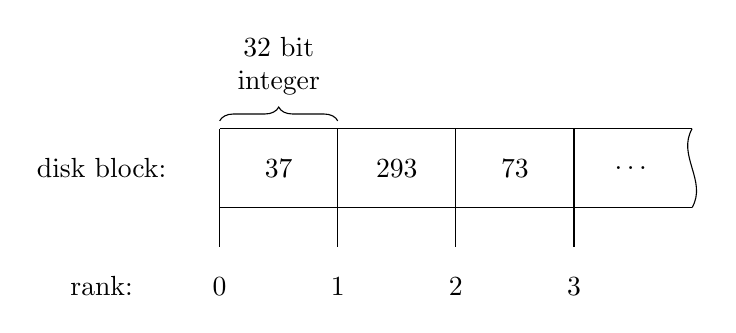
\begin{tikzpicture}[node distance={15mm}, main/.style = {draw, circle}]

    \draw (0,0) -- (6,0);
    \draw (0,1) -- (6,1);
    \draw (0,-0.5) -- (0,1);
    \draw (1.5,-0.5) -- (1.5,1);
    \draw (3,-0.5) -- (3,1);
    \draw (4.5,-0.5) -- (4.5,1);
    \draw[out=60, in=-120] (6,0) to (6,1);

    \node at (0.75, 0.5) {37};
    \node at (2.25, 0.5) {293};
    \node at (3.75, 0.5) {73};
    \node at (5.25, 0.5) {…};

    \node at (-1.5, 0.5) {disk block:};
    \node at (-1.5, -1) {rank:};
    \node at (0, -1) {0};
    \node at (1.5, -1) {1};
    \node at (3, -1) {2};
    \node at (4.5, -1) {3};

    \draw [decorate,decoration = {brace, amplitude=5pt}] (0,1.1) --  (1.5,1.1);
    \node[ align=center] at (0.75, 1.8) {32 bit  \\ integer};

\end{tikzpicture}
    \caption{Position File}
    \label{fig:position_file}
\end{figure}

\begin{figure}
    \centering
    \begin{algorithm}
    \caption{DFS in StoreFunction}
    \begin{algorithmic}
        \label{alg:store_dfs}
        \Procedure{store()}{}
        \While{stack $\neq \emptyset$}
            \If{stack.peekFirst().hasNext()}
                \State $\text{vertex} \gets \text{stack.peekFirst().next()}$
                \If{$\lnot$ positionWriter.alreadyWritten(vertex)}
                    \State position $\gets$ arcWriter.write(vertex)
                    \State positionWriter.write(vertex, position)
                    \State stack.addFirst(neighbors(vertex))
                \EndIf
            \Else
                \State stack.pollFirst()
            \EndIf
        \EndWhile
        \EndProcedure      
    \end{algorithmic}
\end{algorithm}
    \caption{StoreFunction}
    \label{fig:store_function}
\end{figure}

\section{Reading Disk Arcs}

If one wants to get all upwards arcs of rank $i$ one needs take  the upwards position file, retrieve the integer $j$ that is stored at index $i$, and then read the complete block $j$ in the upwards arc file.
One will get an array, containing the requested arcs but also some others.
These arcs are likely to be request next.
Therefore we want to keep them in memory and to do so we use buffers. 
We implemented two buffers a \textit{circular buffer} and a \textit{least recently used buffer} LRU.

\subsection{Circular Buffer}

We implemented a circular buffer to read and cache the DiskArcs at query time.
One might also call it FiFo-buffer, which is correct too. 
The key properties of this buffer are:

\begin{itemize}
    \item The element that resides inside the longest will be overwritten next if a new element is fetched from the disk. So \textit{first in first out} or FiFo.
    \item If the maximum number of elements the buffer is reached it starts to overwrite the elements from the beginning. Therefore \textit{circular} or \textit{ring} buffer.
    \item A element is never \textit{take out}. This means, elements that have been requested and returned will stay inside the buffer until they will be eventually overwritten. 
\end{itemize}
Figure \ref{fig:circular} is simple visualization, for a circular buffer of upward arcs.
There is the DiskArc array that has already been filled with some arcs, a position hash table that contains the last index at which one will find an arc for the requested rank and a write pointer, that tells at which position we have to continue writing when the next cache miss occurs.

\begin{figure}[H]
    \centering
    \begin{tikzpicture}[node distance={15mm}, main/.style = {draw, circle}]

    \draw (0,0) -- (9,0);
    \draw (0,1) -- (9,1);
    \draw (0,-0.5) -- (0,1);
    \draw (1.5,-0.5) -- (1.5,1);
    \draw (3,-0.5) -- (3,1);
    \draw (4.5,-0.5) -- (4.5,1);
    \draw (6,-0.5) -- (6,1);
    \draw (7.5,-0.5) -- (7.5,1);
    \draw (9,-0.5) -- (9,1);

    \node<2-4> at (0.75, 0.5) {a(1,x)};
    \node<2-4> at (2.25, 0.5) {a(1,y)};
    \node<2-4> at (3.75, 0.5) {a(1,z)};
    \node<5-> at (0.75, 0.5) {a(3,x)};
    \node<5-> at (2.25, 0.5) {a(3,y)};
    \node<5-> at (3.75, 0.5) {a(3,z)};
    \node<3-4> at (5.25, 0.5) {a(2,x)};
    \node<5-> at (5.25, 0.5) {a(3,zx)};
    \node<3-> at (6.75, 0.5) {a(2,y)};
    \node<3-> at (8.25, 0.5) {a(2,z)};

    \node at (-1.5, 0.5) {DiskArc[]};
    \node at (-1.5, -1) {index:};
    \node at (0, -1) {0};
    \node at (1.5, -1) {1};
    \node at (3, -1) {2};
    \node at (4.5, -1) {3};
    \node at (6, -1) {4};
    \node at (7.5, -1) {5};
    \node at (9, -1) {size};

    \draw<1>[ -Stealth, ] (0, -4 ) -- node[above, sloped] {writePointer} (0,-1.5);
    \draw<2>[ -Stealth, ] (4.5, -4 ) -- node[above, sloped] {writePointer} (4.5,-1.5);
    \draw<3-4>[ -Stealth, ] (0, -4 ) -- node[above, sloped] {writePointer} (0,-1.5);
    \draw<5-6>[ -Stealth, ] (6, -4 ) -- node[above, sloped] {writePointer} (6,-1.5);



    \node at (-1.5, 2) {positions:};
    \onslide<1>{\node (tab1)  at (3,2) {%
        \begin{tabular}{c }
            \textbf{rank} \\
            \hline
            \textbf{position} \\
        \end{tabular}};
    }
    \onslide<2>{\node (tab1)  at (3,2) {%
        \begin{tabular}{c | c }
            \textbf{rank} & 1  \\
            \hline
            \textbf{position} & 2  \\
        \end{tabular}};
    }
    \onslide<3>{\node (tab1)  at (3,2) {%
        \begin{tabular}{c | c | c }
            \textbf{rank} & 1 & 2 \\
            \hline
            \textbf{position} & 2 & 5 \\
        \end{tabular}};
    }
    \onslide<4>{\node (tab1)  at (3,2) {%
        \begin{tabular}{c | c | c | c}
            \textbf{rank} & 1 & 2 & max(rank) \\
            \hline
            \textbf{position} & 2 & 5 & -1 \\
        \end{tabular}};
    }
    \onslide<5>{\node (tab1)  at (3,2) {%
        \begin{tabular}{c | c | c | c | c}
            \textbf{rank} & 1 & \textcolor{red}{2} & 3 & max(rank) \\
            \hline
            \textbf{position} & 2 & \textcolor{red}{5} & 3 & -1 \\
        \end{tabular}};
    }
    \onslide<6->{\node (tab1)  at (3,2) {%
        \begin{tabular}{c | c | c | c }
            \textbf{rank} & 1 & 3 & max(rank) \\
            \hline
            \textbf{position} & 2 & 3 & -1 \\
        \end{tabular}};
    }

    \onslide<5>{
      \node at (0,-2){\textcolor{red}{remove incomplete edge set from position}};
    }
   

\end{tikzpicture}
    \caption{Circular Buffer for upwards arcs}
    \label{fig:circular}
\end{figure}

If a rank is requested which is already in the buffer, we look up the position in the positions hash table and start iterating with decreasing index from the retrieved position until the start vertex of the arc we read has a different rank than the requested.
If we reach the start of the DiskArc query the iteration index is reset ti the last index of the DiskArc array, such that we continue reading at the end of the DiskArc array.
\\
If the rank we requesting isn't in the hash table we request the containing block from the disk.
We receive an array of DiskArcs that contains all arcs of the requested rank and maybe some more, which are also likely to be requested soon.
At first we insert $-1$ for the request rank into the hash table.
This is because one will not find a DiskArc for every rank one requests.
For instance the vertex with the highest rank will not have any outgoing arcs.
To prevent having such vertices requested from the disk every time the search touches the top of the graph we have a $-1$ in the position table and if that rank is requested we simply return an empty collection.
We iterate the just load DiskArc array.
For each DiskArc we insert the start arc rank into the position table, together with the current position and the disk arc into the array at the current position.
After each insert we increment the positionWriter by $1$.
If we reach the end of the buffer array it is back set to $0$.
\\
As it is possible that we only partly overwrite some arc sets that are already in the buffer, we get the start rank of the arc at the \textit{writePointer} position and remove this rank from the positions table after each disk read invocation.
\\ 
Determine whether a arc set is inside the buffer isn't trivial.
If it's not in position table, it not in the buffer.
If it's in the positions table it is possible that it has been overwritten.
So we check whether at position we retrieve from the table there is actually a arc that starts with the requested rank.
If yes, the buffer contains the arc set, if no it doesn't and we remove that rank from the position table.

\subsection{Least Recently Used Buffer}

With the class \textit{java.util.LinkedHashMap} it is very easy to create a LRU-Buffer.
It provides the possibility to evicted the entry that has been requested longest time ago, if a certain key size has been reached.
In our case it maps ranks to sets of disk arcs.
We can only determine how many disk arc sets we have in memory and disk arc sets do not have always the same size.
Higher rank vertices usually have more arcs as they are of higher degree.
The advantage is, it is very easy to implement and therefore very resilient to programming errors.

\section{The Search}

The search brings all things explained in this chapter together.
At the beginning there are to index graphs initialized the upwards graph $G_\uparrow'(V_\uparrow, A_\uparrow)$ and the downwards graph $G_\downarrow'(V_\downarrow, A_\downarrow)$.
We are looking for the shortest path from the source vertex $v(s)$ to the target vertex $v(t)$.
The vertex set $V_\uparrow$ of the upwards graph $G_\uparrow'(V, A_\uparrow)$ only contains one vertex $v(s)$ and the upward arc set is empty $A_\uparrow = \emptyset$.

The vertex set $V_\downarrow$ of the downwards graph $G_\downarrow'(V_\downarrow, A_\downarrow)$ only contains the $v(t)$ and the arc set is empty $A_\downarrow = \emptyset$.
Looking at graph in figure \ref{fig:lazy_load_vertex} visualizes the upwards search size after initialization.
The ars an vertices in grey are not loaded yet.
\\
As defined earlier in section \ref{sec:dijkstra}, the vertices of the dijkstra query are wrapped in a object called \textit{DijkstraState} which is define in figure \ref{fig:dijkstra_class}.
We now extend this class by one parameter, the \textit{VertexLoader} which you can see in figure \ref{fig:lazy_load_vertex}.
The \textit{VertexLoader} has only one method \textit{addArcs(vertex: Vertex)}.
If you pass a vertex to this method the VertexLoader will take that vertex and attached all its arcs and their end vertices to it.
This happens when the \textit{expandNext()} method in algorithm \ref{alg:disjkstra_algorithm} calls \textit{state.settle()}.
This follows the observation that the arcs of a vertex in dijkstra are only of interest if the query is about to expand this vertex.
\\
The \textit{VertexManager} gets \textit{DiskArc}'s from a \textit{Buffer}.
The buffer can be of any buffer type it only has to implement \textit{arcs(rank: int):Set<DiskArc>} method.
The \textit{VertexManager} is in to responsibility create the arcs and vertices form the \textit{DiskArc}'s it gets.
A \textit{Buffer} contains some type of collection data structure caches \textit{DiskArc}'s.
When the vertex manger requests some arcs the \textit{Buffer} checks whether they are already cached.
If yes it returns them.
If not it will request the arcs from the hard drive.
This whole process is also visualized in figure \ref{fig:lazy_load_vertex}.
\\
After starting the CH-Dijksta as described in algorithm \ref{alg:cchSearch} both $G_\uparrow'$ and $G_\downarrow'$ are alternatingly expanded and the vertices will be attached when needed.
This can be compared to Command \& Conquer or a lot of other real-time strategy video games where you start at a map that is almost completely grey and the map is only load to the position you are plus some padding.

\begin{figure}
    \centering
    \begin{tikzpicture}[node distance={15mm}, main/.style = {draw, circle}]

    \node[rotate=90] at (-0.25,0) {rank};
    \draw [ -Stealth]  (0,-2) -- (0,2);

    %\node[] at (3,3) {Lower Triangles};
    
    \node[main, draw=black!20] (y) at (1, 0) {$y$}; 
    \node[main] (x) [below right of=y] {$x$};
    \node[main, draw=black!20] (z) [right of=z, above of=y] {$z$}; 

    \draw[ -Stealth, draw=black!20] (x) -- (z);
    \draw[ -Stealth, draw=black!20] (x) -- (y);
    
    \draw[ -Stealth, ] ( 2.5 , -1 ) -- node[above, sloped] {settle()} (5,-0.2);

    \begin{class}[text width=0.2\linewidth]{VertexManager}{7,2}
        \operation{+ VertexManager(b: Buffer)}
        \operation{+ addArcs(vertex: Vertex)}
    \end{class}

    \begin{class}[text width=0.2\linewidth]{Buffer}{14,2}
       \operation{+ arcs(rank: int): Set<DiskArc>}
    \end{class}

    \draw [] (13,-3) -- (13,-2);
    \draw [] (15,-3) -- (15,-2);    

    \draw [out=30, in=-210] (13,-2) to (15,-2);    
    \draw [out=-30, in=-150] (13,-2) to (15,-2);    
    \draw [out=-30, in=-150] (13,-3) to (15,-3); 

    \node[] at (14,-2.7) {Disk};

    \draw [ -Stealth] (13,0) to node[above, sloped] {get(0xFF)} (13,-1.9); 
    \draw [ -Stealth] (15,-1.9) to node[above, sloped] {byte[]} (15,0); 

    \draw [ -Stealth ] (9,2) to node[above, sloped] {arcs(x)} (12,2);    
    \draw [ -Stealth ] (12,0.2) to node[above, sloped] {\{a(x,x), a(x,z)\}} (9,0.2);    


    
\end{tikzpicture}
    \caption{lazy load vertex at query time}
    \label{fig:lazy_load_vertex}
\end{figure}


%\begin{figure}
%    \centering
%    \begin{tikzpicture}[node distance={15mm}, main/.style = {draw, circle}]

    \draw (0,0) -- (9,0);
    \draw (0,1) -- (9,1);
    \draw (0,-0.5) -- (0,1);
    \draw (1.5,-0.5) -- (1.5,1);
    \draw (3,-0.5) -- (3,1);
    \draw (4.5,-0.5) -- (4.5,1);
    \draw (6,-0.5) -- (6,1);
    \draw (7.5,-0.5) -- (7.5,1);
    \draw (9,-0.5) -- (9,1);

    \node<2-4> at (0.75, 0.5) {a(1,x)};
    \node<2-4> at (2.25, 0.5) {a(1,y)};
    \node<2-4> at (3.75, 0.5) {a(1,z)};
    \node<5-> at (0.75, 0.5) {a(3,x)};
    \node<5-> at (2.25, 0.5) {a(3,y)};
    \node<5-> at (3.75, 0.5) {a(3,z)};
    \node<3-4> at (5.25, 0.5) {a(2,x)};
    \node<5-> at (5.25, 0.5) {a(3,zx)};
    \node<3-> at (6.75, 0.5) {a(2,y)};
    \node<3-> at (8.25, 0.5) {a(2,z)};

    \node at (-1.5, 0.5) {DiskArc[]};
    \node at (-1.5, -1) {index:};
    \node at (0, -1) {0};
    \node at (1.5, -1) {1};
    \node at (3, -1) {2};
    \node at (4.5, -1) {3};
    \node at (6, -1) {4};
    \node at (7.5, -1) {5};
    \node at (9, -1) {size};

    \draw<1>[ -Stealth, ] (0, -4 ) -- node[above, sloped] {writePointer} (0,-1.5);
    \draw<2>[ -Stealth, ] (4.5, -4 ) -- node[above, sloped] {writePointer} (4.5,-1.5);
    \draw<3-4>[ -Stealth, ] (0, -4 ) -- node[above, sloped] {writePointer} (0,-1.5);
    \draw<5-6>[ -Stealth, ] (6, -4 ) -- node[above, sloped] {writePointer} (6,-1.5);



    \node at (-1.5, 2) {positions:};
    \onslide<1>{\node (tab1)  at (3,2) {%
        \begin{tabular}{c }
            \textbf{rank} \\
            \hline
            \textbf{position} \\
        \end{tabular}};
    }
    \onslide<2>{\node (tab1)  at (3,2) {%
        \begin{tabular}{c | c }
            \textbf{rank} & 1  \\
            \hline
            \textbf{position} & 2  \\
        \end{tabular}};
    }
    \onslide<3>{\node (tab1)  at (3,2) {%
        \begin{tabular}{c | c | c }
            \textbf{rank} & 1 & 2 \\
            \hline
            \textbf{position} & 2 & 5 \\
        \end{tabular}};
    }
    \onslide<4>{\node (tab1)  at (3,2) {%
        \begin{tabular}{c | c | c | c}
            \textbf{rank} & 1 & 2 & max(rank) \\
            \hline
            \textbf{position} & 2 & 5 & -1 \\
        \end{tabular}};
    }
    \onslide<5>{\node (tab1)  at (3,2) {%
        \begin{tabular}{c | c | c | c | c}
            \textbf{rank} & 1 & \textcolor{red}{2} & 3 & max(rank) \\
            \hline
            \textbf{position} & 2 & \textcolor{red}{5} & 3 & -1 \\
        \end{tabular}};
    }
    \onslide<6->{\node (tab1)  at (3,2) {%
        \begin{tabular}{c | c | c | c }
            \textbf{rank} & 1 & 3 & max(rank) \\
            \hline
            \textbf{position} & 2 & 3 & -1 \\
        \end{tabular}};
    }

    \onslide<5>{
      \node at (0,-2){\textcolor{red}{remove incomplete edge set from position}};
    }
   

\end{tikzpicture}
%    \caption{Circular Buffer}
%    \label{fig:circular_buffer}
%\end{figure}
